\chapter{Risultati Sentiment Analysis con il modello \textit{Feel-It}}
L’ultima fase del lavoro riguarda l'analisi delle emozioni e dei temi più ricorrenti all'interno dei tweet scritti sul team app Immuni, in modo tale da comprendere meglio i problemi legati a questi app e gli aspetti su cui gli utenti discutono maggiormente.

Come illustrato in \ref{sec: sent_an}, per eseguire la Sentiment Analysis su questo corpus per classificare sia le emozioni che la tipologia di sentimenti, analizzando quindi la polarità, si utilizzerà il Modello \textit{Feel-It}

In particolare, per questa indagine si è scelto di analizzare le emozioni a due livelli di granularità differenti, applicando prima il modello a tutto il corpus e successivamente ai tweet scritti in due diversi periodi temporali: quelli scritti nel 2020 (6397 tweet) e quelli scritti nel 2021 (3387 tweet),  poiché la raccolta dei dati è avvenuta in un periodo molto lungo, in modo tale da evidenziare eventuali cambiamenti riguardo alle emozioni provate dall'utente riguardo all'utilizzo di Immuni.

\section{Analisi della polarità}
Innanzitutto, si è provveduto all'analisi della \textbf{polarità}, utilizzando il modello predittivo \textit{sentiment\_classifierier}, il quale estrarre dai dati i sentimenti, classificandoli in positivi e, negativi, applicandolo prima sull'intero insieme di tweet e successivamente sui due periodi temporali.
\begin{table}[H]
\centering
    \begin{tabular}{|l|c|c|c|}
    \hline
    \rowcolor[HTML]{DAE8FC} 
                       & \textbf{Tweet Totali} & \textbf{Tweet 2020} & \textbf{Tweet 2021} \\ \hline
    \textit{Negativi}    & 8580    & 5656  & 2924    \\ \hline
    \textit{Positivi}     & 1204   & 741   & 463                 \\ \hline
    \end{tabular}
    \caption{Risultato della classificazione effettuata dal Modello Feel-It sui tweet totali e di quelli scritti nel 2020 e 2021}
    \label{table: ris_fellit}
\end{table}
La tabella \ref{table: ris_fellit} mostra come in tutti e tre i corpora la maggior parte dei tweet siano negativi, sinonimo che in generale l'attitudine degli utenti nei confronti dell'App Immuni sia di natura negativa, un dato che giustificherebbe il progressivo fallimento dell'applicazione dovuto alla non coinvolgimento da parte degli utenti e in generale alla scarsa promozione dell'app da parte del Governo e alla crisi interna del Governo italiano che nel 2021 ha visto la caduta del Governo Conte avvenuta il 26 gennaio 2021 con le dimissioni di Giuseppe Conte e l'arrivo al potere del Presidente Mario Draghi, il quale però non si è ancora espresso sull'utilizzo dell'app.


\section{Analisi dei sentimenti}
Successivamente, si è scelto di analizzare le emozioni provate dagli utenti nel momento in cui pubblicano un tweet per esprimere la propria opinione sul tema App Immuni. Per eseguire questa indagine, è stato utilizzato un altro modello predittivo di Feel-It, il modello \textit{emotion\_classifier} che annota il corpus secondo 4 emozioni: paura, rabbia, gioia e tristezza. 
\begin{table}[H]
\centering
\begin{tabular}{|l|c|c|c|}
\hline
\rowcolor[HTML]{DAE8FC} 
                   & \textbf{Tweet totali} & \textbf{Tweet 2020} & \textbf{Tweet 2021} \\ \hline
\textit{Rabbia}    & 6249                  & 4021                & 2228                \\ \hline
\textit{Paura}     & 2507                  & 1779                & 728                 \\ \hline
\textit{Felicità}  & 721                   & 433                 & 288                 \\ \hline
\textit{Tristezza} & 307                   & 164                 & 143                 \\ \hline
\end{tabular}
\caption{Risultati della classificazione delle emozioni estratte dai tweet totali e da quelli pubblicati nel 2020 e 2021}
\label{tab: emotions}
\end{table}
I risultati derivati dall'applicazione di questo modello e illustrati nella tabella \ref{tab: emotions}, mostrano come le emozioni più rilevanti siano la rabbia e la paura, entrambe emozioni negative, che confermano quindi una polarità negativa degli utenti come si era visto precedentemente, e che in un certo senso sono legate al tema App Immuni, che ha spesso creato dibattito su temi riguardanti non solo la salute, ma anche la privacy e la cessione di dati sensibili, due aspetti che possono essere collegati al sentimento della paura e della rabbia da parte degli utenti. 
\begin{figure}[H]
	\centering
	\subfloat[]
	{
		\label{sent_an_2020}
		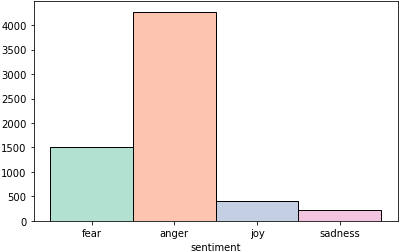
\includegraphics[width=.47\textwidth]{img/sentAnalysis2020.png}
	}
	\quad
	\subfloat[]
	{
		\label{sent_an_2021}
		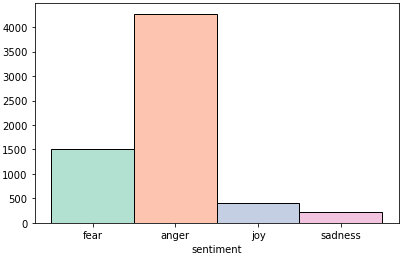
\includegraphics[width=.47\textwidth]{img/sentAnalysis2021.png}
	}    
	\quad
	\setlength{\belowcaptionskip}{-10pt}
	\caption{Distribuzione dei sentimenti all'interno dei tweet pubblicati nel 2020 (a destra), e nel 2021 (a sinistra)}
	\label{fig: sentan}
\end{figure}
Tuttavia, queste due emozioni si distribuiscono in maniera diversa all'interno dei due anni, diminuendo progressivamente nel 2021, un aspetto che può essere giustificato dal fatto i dati raccolti nel 2021 (Figura \ref{sent_an_2021}) sono minori rispetto a quelli del 2020  (Figura \ref{sent_an_2020}), fenomeno dovuto al fatto che con il passare del tempo l'app Immuni è andata pian piano in disuso per motivi sia politici, dovuti alla già citata mancata organizzazione e promozione, che sanitari grazie all'arrivo di misure di prevenzione più efficaci contro la diffusione del virus, come i vaccini.
Tuttavia, è possibile notare anche la presenza di una piccola percentuale di tweet classificati come \textit{gioia}, sintomo che alcuni utenti siano favorevoli all'utilizzo dell'applicazione, una percentuale che però non riesce a consolidare il successo dell'applicazione.

\begin{figure}[H]
	\centering
	\subfloat[]
	{
		\label{wordcloud_gioia}
		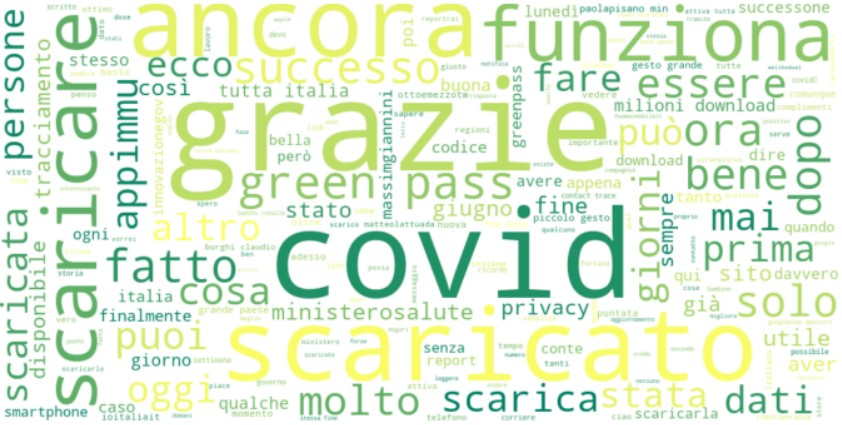
\includegraphics[width=.47\textwidth]{img/wordcloud_parole_gioia.jpg}
	}
	\quad
	\subfloat[]
	{
		\label{wordcloud_rabbia}
		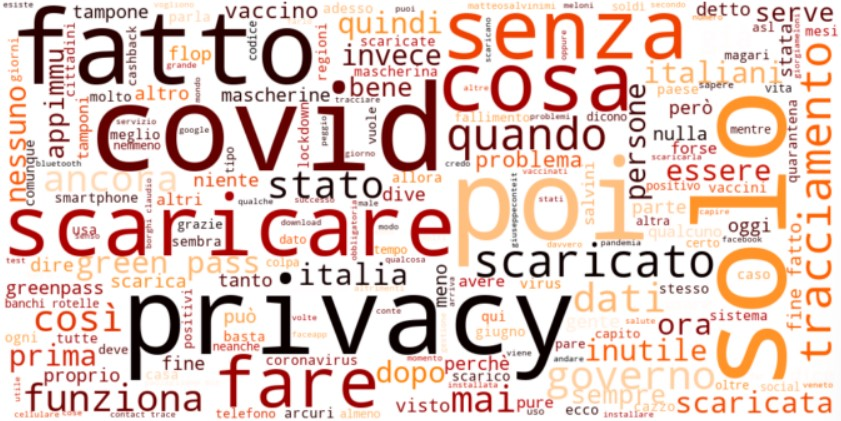
\includegraphics[width=.47\textwidth]{img/wordcloud_parole_rabbia.jpg}
	}    
	\quad
	\setlength{\belowcaptionskip}{-10pt}
	\caption{Parole più utilizzate nei tweet classificati come '\textit{goia}' (\ref{wordcloud_gioia}) e '\textit{rabbia}' (\ref{wordcloud_rabbia})}
	\label{fig: wordclouds}
\end{figure}

Infine, si è scelto di esaminare ulteriormente le emozioni estratte dai tweet, analizzando le parole più frequenti all'interno dei tweet classificate con le emozioni positive (corrispondenti alla gioia, Figura \ref{wordcloud_gioia}) e tra quelle negative quelle legate alla rabbia (Figura \ref{wordcloud_rabbia}).
Per semplificare l'analisi dei risultati si è scelto di rappresentare queste parole sotto forma di \textit{wordcloud}, una tecnica di rappresentazione visiva funzionale alla visualizzazione delle parole chiave più utilizzate grazie all'utilizzo di colori e dimensioni grafiche diverse che servono per identificare l'importanza di un termine all'interno di un insieme di parole. Nonostante nel caso della gioia tra le parole più ricorrenti compaiano 'grazie', 'funziona', nel caso della rabbia, che come si è visto è il sentimento prevalente all'interno del corpus, si evidenzia come la maggior parte degli utenti pubblichi tweet con argomenti legati soprattutto alla non fiducia nella campagna promozionale delle istituzioni nei confronti di Immuni, un fenomeno che potrebbe essere rappresentato dal termine "governo", e nel tracciamento eseguito utilizzando dati sensibili, un dato che viene giustificato dalla forte presenza di termini come \textit{privacy}, e \textit{dati} che come si è osservato anche nelle analisi precedente sono due dei termini che rappresentano i problemi maggiori legati a Immuni suscitando anche un forte dibattito tra gli utenti.

%In entrambi i casi le parole più frequenti, rappresentate utilizzando un \textit{font} più grande, sono tutte legate alle varianti del nome dell'applicazione (\textit{App, AppImmuni, ImmuniApp, Immuni}). 

